\documentclass[12pt, oneside]{article}   	% use "amsart" instead of "article" for AMSLaTeX format
\usepackage{geometry}                		% See geometry.pdf to learn the layout options. There are lots.
\geometry{letterpaper}     
\geometry{margin=1.5in}        		% ... or a4paper or a5paper or ... 
%\geometry{landscape}                		% Activate for for rotated page geometry
%\usepackage[parfill]{parskip}    		% Activate to begin paragraphs with an empty line rather than an indent
\usepackage{graphicx}				% Use pdf, png, jpg, or eps§ with pdflatex; use eps in DVI mode
\usepackage{times}								% TeX will automatically convert eps --> pdf in pdflatex		
\usepackage{amssymb}
\usepackage{setspace}
\doublespacing



\title{ORAM paper}
\author{Akiva Gordon, Krishna Suraj}

\date{}							% Activate to display a given date or no date

\begin{document}
\maketitle

\begin{abstract}
In today's world, an ever-increasing amount of data is being stored online in the "cloud" - external, untrusted servers. Considering the importance of such data to users, businesses, and organizations, it is necessary to protect data from mishandling and exploitation from those servers. While current encryption schemes can protect the actual data on a server from being read, a user's access pattern to files on a server is vulnerable. Oblivious RAM (ORAM) is a cryptographic primitive that hides a user's access pattern metadata from untrusted servers. In this work, we discuss and analyze various ORAMs. We first provide an explanation of the various tree-based ORAM algorithms, including Constant Communication ORAM (C-ORAM), a constant-bandwidth, high-efficiency algorithm. We then provide an experimental analysis of C-ORAM using our implementation of the algorithm in Python 2.7. Using data from our experimental analysis, we determine runtime as well as  optimal bucket size and eviction frequency based on many accesses to our ORAM implementation.

\end{abstract}


\section{Introduction}
Since the advent of the ``internet age", the number of files and data being created grows exponentially every year. Users store an ever-increasing amount of data on the internet using cloud services such as Google Drive and Dropbox. Even more significantly, thousands of businesses store private data on the cloud using services such as Amazon Web Servers (AWS). With an ever-increasing amount of data being created and stored on the cloud, a user's privacy and anonymity in the digital world is becoming more important than ever before. To protect private data and enterprise secrets, users and businesses are increasingly concerned with the threat of data theft.

Important data on the cloud should be encrypted, such as in online transfers (e.g., PayPal). While current encryption schemes do a good job of protecting actual data, a user's metadata created when accessing and operating on data is still unprotected. For example, if a business were to store encrypted data on external or rented servers (e.g., Amazon Web Servers) the untrusted server could still see which files are being accessed, the frequency of accesses, and the time of such accesses. This metadata, or access pattern, is important to protect because otherwise an untrusted server may deduce information about the files themselves. For example, if certain files are accessed more often, the server may deduce that they are important files. Also, if certain files are accessed a lot before a certain data (e.g., tax day), the server may conclude that those files serve a certain purpose (e.g., a user's private tax returns).

Oblivious RAM (ORAM) is a cryptographic primitive that enables a user to store data on an untrusted server while maintaining data obliviousness - that is, the server cannot gain information about the user's access pattern of their files. ORAM preserves these access patterns and allows the user to conceal their activity from the server. Thus, ORAM grants a user essential privacy online.%repetitive, add what it protects instead

%Ling: would be nice if you can add a little transition here, like a very very brief history of ORAM

In this work, we examine Constant Communication ORAM (C-ORAM)~\cite{C-ORAM}, a recent ORAM scheme using server computation that builds upon Onion ORAM~\cite{OnionORAM}. C-ORAM reduces the overall bandwidth of Onion ORAM by introducing novel eviction techniques that reduce the amount of encryption layers needed from Onion ORAM.
%\subsection{}



\section{Previous work}

\subsection{Previous tree-based ORAM schemes}
Initially proposed by Goldreich and Ostrovsky~\cite{TODO}, Oblivious RAM has long remained in the theoretical domain, with bandwidth being a limiting factor preventing the practical adoption of ORAM. Path ORAM~\cite{TODO} demonstrated the use of a tree data structure for ORAM, a significant step forward closer the theoretical asymptotic limit for ORAM - on the order of $\log N$. Path ORAM introduced the use of a binary tree to store an ORAM structure. Units of data called ``blocks" are stored in ``buckets" - the nodes of the binary tree. Each bucket occupies one whole node of the binary tree. Each data block has a unique path to a leaf node on the tree. A data access in Path ORAM consists of a request to the position map, which stores a list of data blocks and their corresponding paths. Then, the user pulls the entire contents of the path into the ``client space." The client space is assumed to be fully secure. The selected data block is operated on using a read/write operation. All other blocks are placed back on their original paths. The accessed block is assigned a new path to maintain obliviousness, and placed at the bucket which is the lowest intersection on the tree of the old and new paths. Ring ORAM, another tree-based ORAM, is an optimization of Path ORAM. One improvement is the reduction of bandwidth use during an access. If a tree has $l$ levels and each bucket has $z$ blocks, Ring ORAM pulls only $l$ blocks to the client, rather than $l*z$ blocks in Path ORAM. It does this by pulling only one block from each bucket on the path, rather than all blocks on a path. When traversing a path during an access, if the desired block is present in the current bucket, it is retrieved to the client and replaced with a dummy block - a block with meaningless, randomly generated data. If not, a reserved ``dummy" block, which is intended for the purpose of retrieval is sent back. The dummy blocks are discarded on the client side. Figure \ref{fig:ringaccess} shows the process of selecting one block from each bucket in Ring ORAM.

\begin{figure}[h!]
  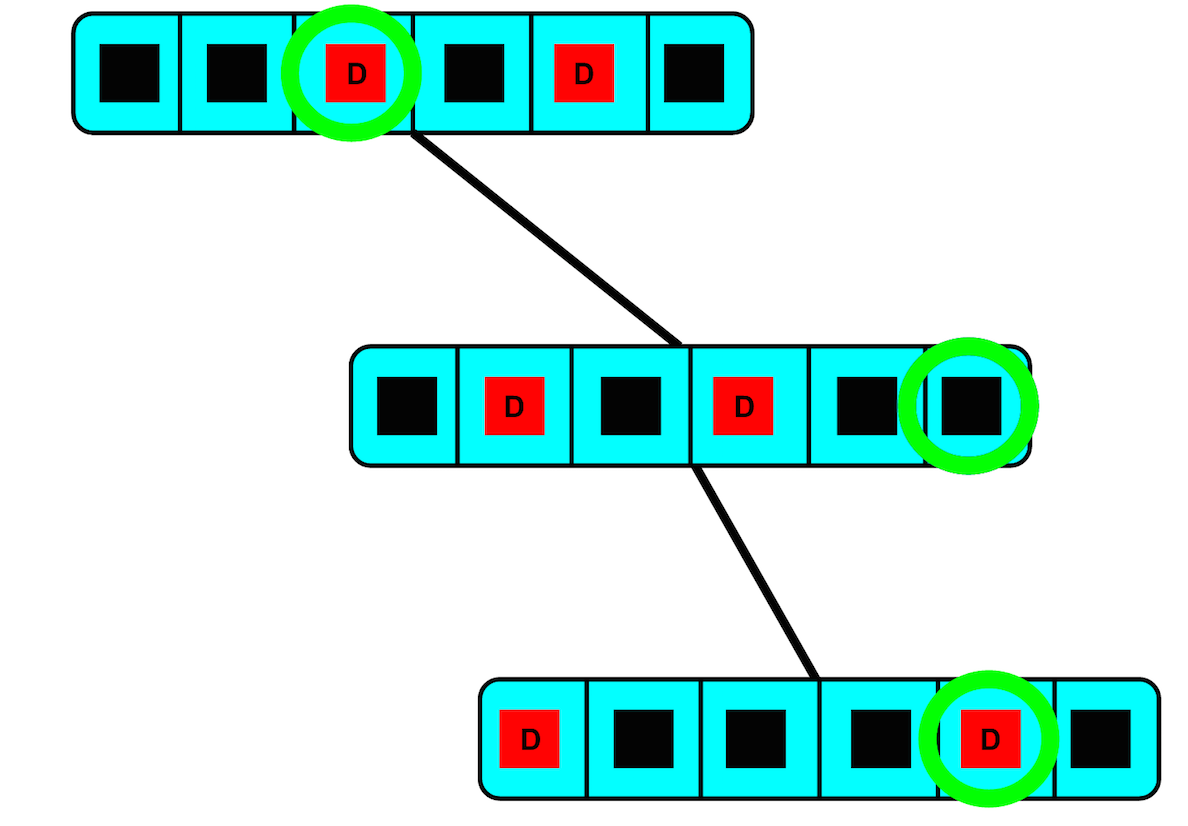
\includegraphics[width=\linewidth]{ringaccess1.png}
  \caption{Ring ORAM access. The circled blocks are selected. The buckets which do not contain the target block (levels 1 and 3) send back a reserved dummy block}
  \label{fig:ringaccess}
\end{figure}


There are two changes to the eviction process in Ring ORAM.  First, eviction only occurs after every $A$ accesses, in which $A$ is a user-selected parameter. Second, instead of replacing blocks in the tree along the path they were retrieved from, they are replaced along a path chosen through reverse lexicographic order. Although $A$ and the path of eviction are public, they are deterministic and therefore independent of the block or the action taken, so they do not compromise the security of the system. Figure \ref{fig:rlo} shows the process of selecting eviction paths in Ring ORAM, Onion ORAM, and C-ORAM.


\begin{figure}[h!]
  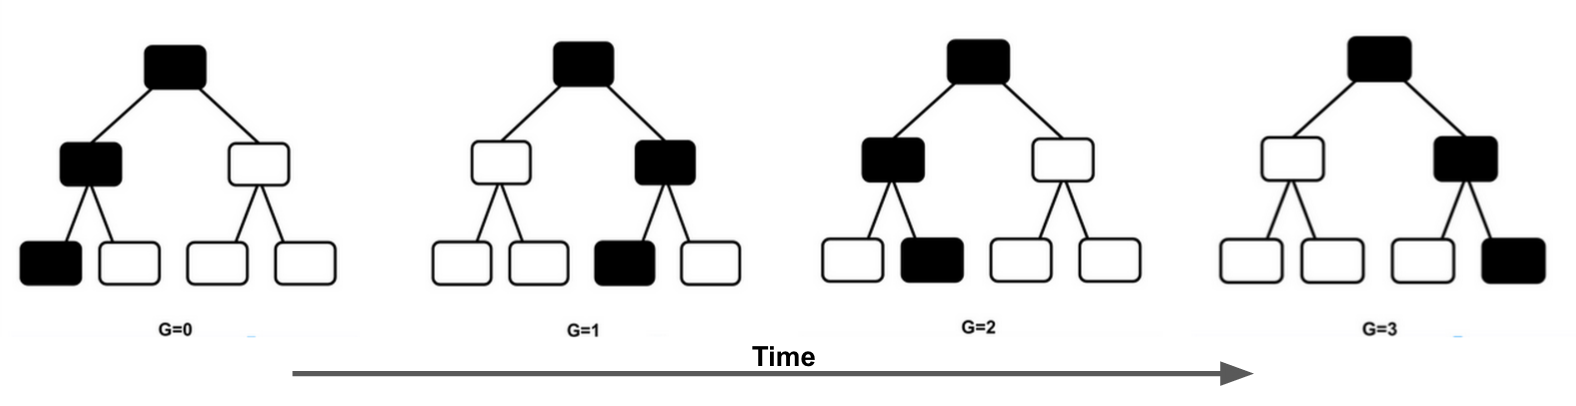
\includegraphics[width=\linewidth]{rlo.png}
  \caption{Reverse lexicographical order balances the tree through standardized evictions.}
  \label{fig:rlo}
\end{figure}


\subsection{Onion ORAM}
Onion ORAM implemented, using additively homomorphic encryption, the idea of having the server conduct some computations for the user rather than all computation being conducted on the user's end. Although earlier works have used server computation, Onion ORAM is the first to achieve constant bandwidth. all data is encrypted and shuffled on the server, so it is very counterintuitive that the server can do any useful work to access or retrieve the files. The server computes on an encrypted bit string and returns a number of blocks, one "real" block and the rest "dummy" blocks so the server cannot know which block the user wants. The dummy blocks are discarded. This is called a Private Information Retrieval. To conduct a private information retrieval, the client first extracts the information to what path the desired data block is on using the position map. Using the path, the client sends an encrypted bit string to the server which the server computes on the eviction path to return one block from each bucket. The server will return dummy blocks from all buckets except for the bucket where the desired data block is, when it will return the data block itself. On the client side, the dummy blocks are discarded and the data block is subject to either a read or write operation. The block is then pushed back on to the Onion ORAM tree at the root node. 

\subsection{Onion ORAM Eviction}
Evictions in Onion ORAM do not happen every access to the block, but periodically. The parameter $A$ describes this frequency. The eviction step of Onion ORAM consists of all blocks on a certain eviction path being pushed all the way to the leaf nodes of the tree. Each step of this eviction, a new layer of additively homomorphic encryption must be added to the data as it is additively merged with the data below it. This, after many operations, will result in a very long cipher text and a very high bandwidth cost. Thus, the encryption bottleneck is very costly in terms of the server's computation efficiency. After all the data is evicted to the leaf, the non-leaf parent blocks are cleared, resulting in an empty path save the leaves. Onion ORAM uses a very costly encryption scheme - Damgard Jurik - discussed in the Onion ORAM paper. Encryption in Onion ORAM is the bottleneck, resulting in a poor computational efficiency although a constant bandwidth efficiency successfully breaks the $\log N$ bound previously suggested to be the lower bound for ORAM bandwidth efficiency.

\section{C-ORAM}
Constant communication ORAM (C-ORAM), proposed by Moataz, Mayberry, and Blass seeks to replace the homomorphic eviction routine in Onion ORAM with a cheaper eviction sequence that replaces the homomorphic multiplications of Onion ORAM while maintaining security. This removes the need for Onion ORAM's layers of encryption and reduces the minimum block size and server computation cost. We start by introducing the C-ORAM process and then provide an experimental analysis.

\subsection{Accesses}

To perform a data access in C-ORAM, the client first retrieves a location tag for the block from the position map (an additional data structure that stores the locations of the specific blocks. This tag defines the path in which the unique data block is located on. Then, the client conducts a Private Information Retrieval applied to each bucket on the path. A data retrieval is performed on every bucket on the specific path to maintain obliviousness - this way, the server does not know which specific data block is being accessed. The client thus retrieves the data block and can perform read or write operations on it in the secure client space. Afterwards, the client can perform a private write into the tree, placing the data block into the root of the C-ORAM tree. C-ORAM accesses are identical to Onion ORAM accesses.

\subsection{Evictions}
In C-ORAM, an eviction only happens every $A$  operations, where $A$ is a parameter. A path to evict along is, like Onion ORAM, chosen following reverse lexicographical order. First, the root bucket, which is assumed to be empty (e.g.. filled with $E (0)$'s (encryptions of zeros), is accessed and written to with encrypted data. This is a normal private write operation.

Constant Communication ORAM differs from Onion ORAM in its eviction step. C-ORAM eviction occurs when the data in each bucket on the selected path merges its data with its two child buckets. These merges are called Oblivious Merges and are detailed in the following section. Only one of these buckets will be on the desired path, so the ``destination" bucket's ``sibling" will have data blocks that are not intended for it but for the destination bucket. Likewise, the destination bucket will have data blocks from the parent bucket that were meant for its sibling bucket. These blocks are called ``noisy" blocks and are functionally useless and disposable since an exact copy of the data exists elsewhere. After every bucket on the path has been merged with its two children, the leaf buckets evicted to will have all the data, so the parent buckets along the eviction path are cleared - e.g., filled with $E (0)$'s. This completes an eviction in C-ORAM. Before a C-ORAM eviction, the sibling buckets of the eviction path are given to be empty except for the leaves. After an eviction, all the non-leaf buckets on the path are empty while the sibling buckets are not. After a certain number of operations, the leaf buckets are also downloaded and its noisy blocks are cleared (to prevent overflow). Figure \ref{fig:c-evict} shows the process of eviction. 


\begin{figure}[h!]
  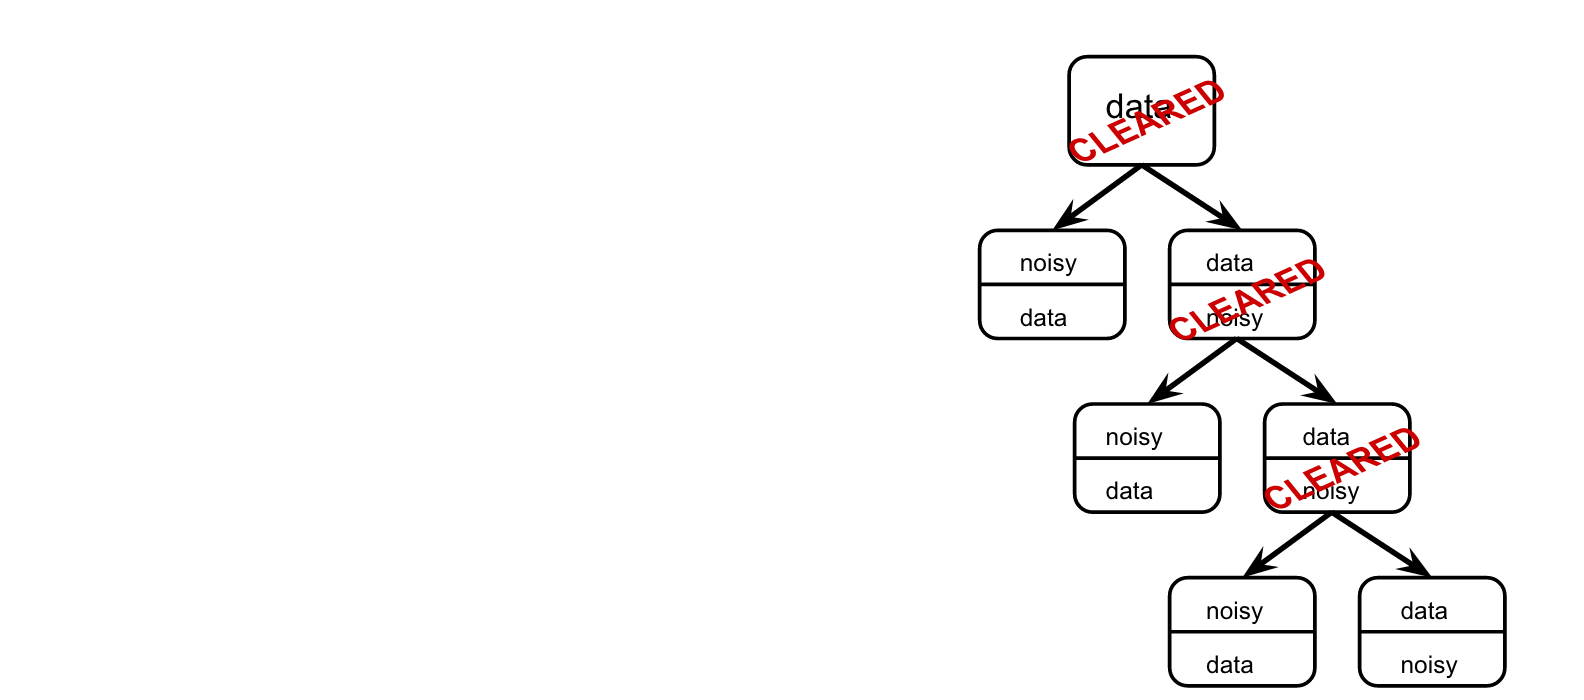
\includegraphics[width=\linewidth]{c-evict.png}
  \caption{Shows the eviction pattern down a particular path in C-ORAM. Although all the data being pushed down to children buckets by parent buckets are identical, noisy blocks on the eviction path are relevant data to their sibling buckets, and vice versa.}
  \label{fig:c-evict}
\end{figure}


\subsection{Oblivious Mergings}
Oblivious Merging is a method that combines two given buckets in a secure method using server computation. It permutes two buckets so that they are obliviously ``lined up" and combined into a single bucket. Rather that just appending the data in one bucket to the end of another bucket, oblivious merging saves spaces by``overlapping" the two buckets. Since noisy blocks are functionally useless, the buckets are permuted so that real data blocks in one bucket line up with either noisy blocks in the other bucket, and vice-versa. For example, in a merging of buckets $A$ and $B$, the $i$th position in bucket $A$ - given to be a real block - will line up with either a noisy block or an zero-encrypted block in position $i$ in bucket $B$. Thus, when the buckets are simply combined, the real blocks are prioritized and preserved and the noisy or zero-encrypted blocks with which they line up with are discarded, losing no information. Figure \ref{fig:merge} shows the process of oblivious merging. 

\begin{figure}[h!]
  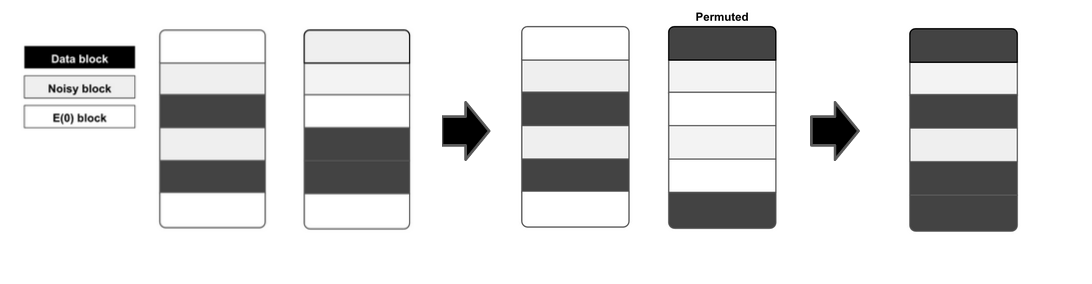
\includegraphics[width=\linewidth]{merge}
  \caption{Two buckets are permuted so ``real" data blocks (in black) are lined up with either noisy blocks (in grey) or $E (0)$ blocks (in white). Thus, merging the two buckets while preserving real data blocks results in no loss of data.}
  \label{fig:merge}
\end{figure}

A main concern with oblivious merging is the security of the permutation conducted by the server to obliviously line up the two buckets. Since C-ORAM's security proof is not intuitive, we provide an intuitive explanation: if bucket $A$ is randomly permuted and bucket $B$ is permuted to fill the spaces in bucket $A$, bucket $B$'s permutation must also be secure. To elaborate: considering Figure \ref{fig:merge}, the left bucket is assumed to be randomly permuted - that is, the server does not know the locations of specific real, noisy, or $E (0)$ blocks in the bucket. Thus, the left bucket is secure. The right bucket is permuted so that real blocks line up with either noisy blocks or $E (0)$ blocks to prevent a loss of information. This second permutation must be secure and as random as the orientation of the left bucket because it is dependent on the left bucket. Thus, intuitively, we come to an understanding that the oblivious merge operation is secure.

A second concern for C-ORAM is that during repeated oblivious merging, the data and noisy blocks will eventually exceed the storage space of the bucket and the bucket will ``overflow." Thus, it is necessary to determine a minimum size bound at which the bucket does not overflow. Mayberry et al. devises a theoretical proof for this in their C-ORAM proposition work. We address the bound using experimental methods in our tests, outlined below in our contributions.




\section{Our Contributions}

In our project, we created a simplified C-ORAM protocol (eliminating the encryption for testing purposes). We tested the merging eviction protocol for consistency and loss of data:

\subsection{Our Results}

We ran tests with ORAMs ranging from $10$ to $15$ layers with bucket sizes ranging from $500$ to $10000$.

In our tests, it became clear that the speed of the algorithm is asymptotically dependent on the number of blocks already in the tree. This does technically support the constant bandwidth requirement, seeming to be dependent on the constant bucket size, rather than the number of blocks added. However, it will always be true that the program will shuffle and re-align buckets more quickly when fewer real blocks are present.

\begin{figure}[h!]
  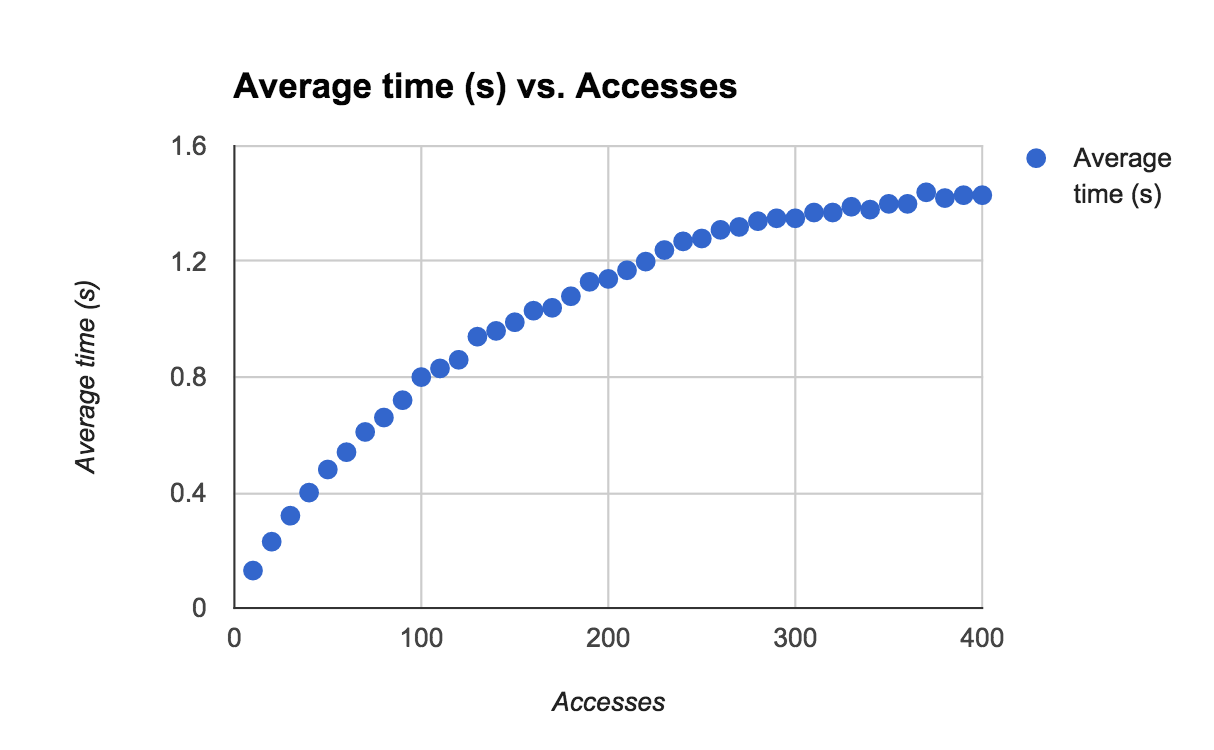
\includegraphics[width=\linewidth]{runtimegraph}
  \caption{}
  \label{fig:runtimegraph}
\end{figure}


We were alarmed to learn that bucket overflow errors occurred quite quickly if more than 10% of the bucket This presents a major problem for storing many blocks. To correct for this issue, it is necessary to subdivide evictions if the client storage has a large number of blocks. 

In addition, noisy blocks must be cleaned from the tree as they will quickly accumulate in the leaves if not dealt with otherwise.

In our protocol, we cleaned the leaf of the eviction path to prevent the tree from filling with noisy blocks, but noisy blocks still accumulated quite quickly in higher layers of the tree, resulting in overflows. The only feasible response to this problem is the constant (or near-constant) removal of noisy blocks from the tree, however, this results in a major compromise of security, and invalidates the primary purpose of the noisy blocks to enable higher security without astronomical bandwidth requirements. We propose that, to reduce this potential for error, we clean a random number of noisy blocks from each bucket during eviction (this process takes negligible time in comparison to the actual eviction).

Without loss of security, we were able to randomly align the merging buckets by only re-ordering one bucket. This requires half the bandwidth of the stated protocol which re-orders both buckets. However, since re-ordering the first bucket is akin to shuffling it randomly, and it is already randomly ordered, no security is lost by re-ordering only one bucket.

\bibliographystyle{abbrv}
\bibliography{ORAM_paper}


\end{document}  
